.% book example for classicthesis.sty
\documentclass[11pt,a5paper,footinclude=true,headinclude=true]{scrbook} % KOMA-Script book
\synctex=1
\usepackage[T1]{fontenc}
\usepackage{lipsum}
\usepackage[linedheaders,parts,pdfspacing]{classicthesis} % ,manychapters
%\usepackage[osf]{libertine}
\usepackage{fancyhdr}
\usepackage{datetime}
\usepackage{amsthm}
\usepackage[utf8]{inputenc}
\usepackage[swedish]{babel}
\usepackage[style=apa,authoryear,backend=biber,natbib=true]{biblatex}
\usepackage{graphicx}

%\usepackage{titlesec}
%\titlespacing*\section{0pt}{12pt plus 4pt minus 2pt}{0pt plus 2pt minus 2pt} % storlek på padding efter \section
%\titlespacing*\subsubsection{0pt}{12pt plus 4pt minus 2pt}{0pt plus 2pt minus 2pt}

%\usepackage{polyglossia}
%\setmainlanguage{italian}
%\PolyglossiaSetup{italian}{indentfirst=false}


%grekiska
\usepackage[LGR,T1]{fontenc} \usepackage[utf8]{inputenc}
\newcommand{\textgreek}[1]{\begingroup\fontencoding{LGR}\selectfont#1\endgroup}
%/grekiska

\usepackage{lipsum,etoolbox}
\AtBeginEnvironment{quote}{\small}% Step font down one size relative to current font.
\AtBeginEnvironment{quote}{\vspace{-.25\baselineskip}}% Stuff before {quote}
\AtEndEnvironment{quote}{\vspace{0\baselineskip}}% Stuff after {quote}


%referenser
\graphicspath{ {/home/anon/Dropbox/nth001/images/} }
\addbibresource{/home/anon/Dropbox/klassiskmodern/bibliography.bib}

% datum och tid i footer och numrering
\fancyhf{}
\fancyfoot[L]{\scriptsize{Utkast: \today\ \currenttime}}
\fancyfoot[R]{\scriptsize{\thepage}}
\pagestyle{fancy}



\begin{document}
\booktitle{\begin{center}
\thispagestyle{empty}
\begin{LARGE}
Teoretiska och historiska perspektiv på naturvetenskap\\

\end{LARGE}

\bigskip
Läsguide och akademiskt skrivande

\bigskip
\bigskip
\bigskip

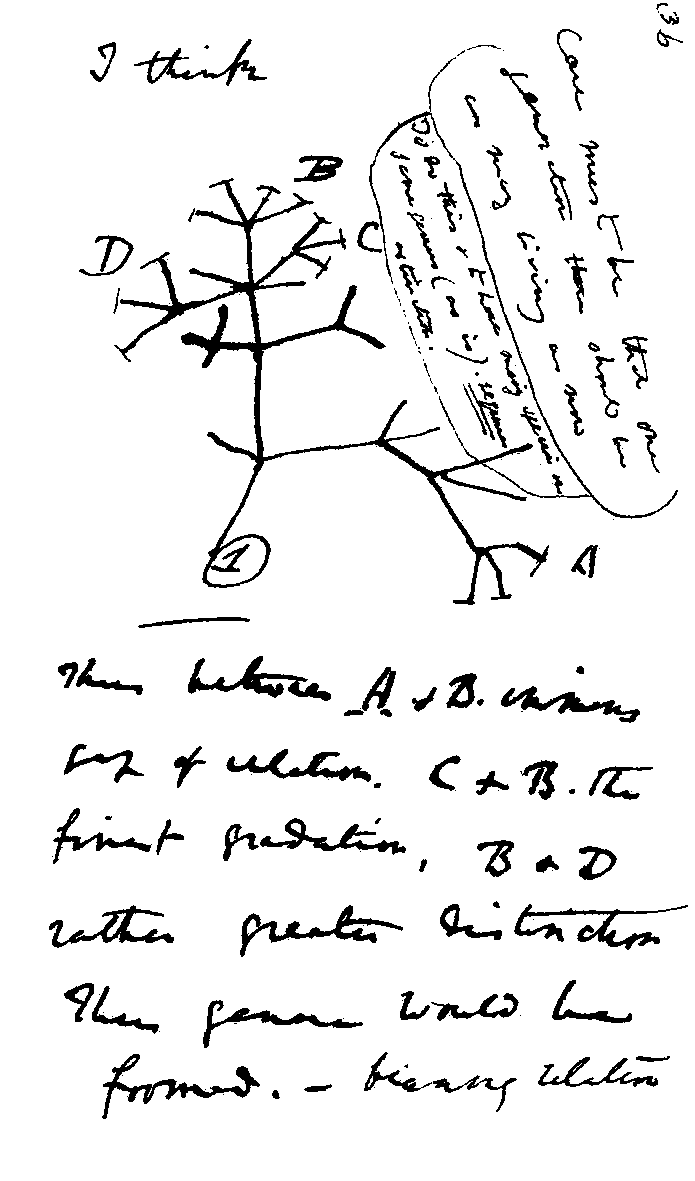
\includegraphics[scale=.5]{Darwin_tree}

\begin{tiny}

\noindent Bild: Charles Darwin (1837) \emph{First Notebook on Transmutation of Species}
\end{tiny}


\end{center}
\noindent Christopher Kullenberg

\noindent \href{https://github.com/christopherkullenberg/nth001}{https://github.com/christopherkullenberg/nth001}

\noindent Licens: GPLV3

%	\pagestyle{scrheadings}
%	\manualmark
%	\markboth{\spacedlowsmallcaps{\contentsname}}{\spacedlowsmallcaps{\contentsname}}

	\tableofcontents
	\thispagestyle{empty}

%	\automark[section]{chapter}
%	\renewcommand{\chaptermark}[1]{\markboth{\spacedlowsmallcaps{#1}}{\spacedlowsmallcaps{#1}}}
%	\renewcommand{\sectionmark}[1]{\markright{\thesection\enspace\spacedlowsmallcaps{#1}}}

    % use \cleardoublepage here to avoid problems with pdfbookmark
    %\cleardoublepage\part{Epistemologi}


\part{Läsguide}

    \chapter{Vetenskapsfilosofi}
		\pagenumbering{arabic} 





     \chapter{Vetenskapshistoria}
     
     \chapter{Vetenskapssociologi}

     \chapter{Teknovetenskaperna}

     \chapter{Genus och vetenskap}

     \chapter{Forskningsetik}
     
     \chapter{Forskningspolitik}
                                      



%	\include{multiToC}
 %   \appendix
 %   \cleardoublepage\part{Appendix}
 %   \chapter{Appendix Chapter}
 %   \lipsum[1]
%
 %   \section{A Section}
  %  \lipsum[1]

\part{Akademiskt skrivande}


    \chapter{Referenser och röstseparering}
    
    \chapter{Röd tråd och stringens}
        
    \chapter{Vetenskapligt språk}
            
    \chapter{Revisioner och redigering}
    
    
    

\printbibliography
\end{document}
